\begin{activity} \label{PA:10.11} In the following questions, we apply the recently-developed Chain Rule in several different contexts.
  \ba
  \item Suppose that we have a function $z$ defined by $z(x,y) = x^2+xy^3$.  In addition, suppose that $x$ and $y$ are restricted to points that move around the plane by following
  a circle of radius $2$ centered at the origin that is parameterized by
    $$
    x(t) = 2\cos t,
    \hspace*{20pt}
    \mbox{and}
    \hspace*{20pt}
    y(t) = 2\sin t.
    $$
%    \begin{itemize}
%    \item What is the position when $t=\pi/4$?
%    \item What are the partial derivatives $\frac{\partial z}{
 %       \partial x}$ and $\frac{\partial z}{\partial y}$ at this
%      point? 
    Use the Chain Rule to find the resulting instantaneous rate of change $\frac{dz}{dt}$.  
%    \end{itemize}
      
  \item Suppose that the temperature on a metal plate is given by
    the function $T$ with 
    $$
    T(x,y) = 100-(x^2 + 4y^2),
    $$
    where the temperature is measured in degrees Fahrenheit
    and $x$ and $y$ are each measured in feet. 
    
    \begin{enumerate}[i.]
    \item Find $T_x$ and $T_y$.  What are the units on these partial
      derivatives?    
    \item Suppose an ant is walking along the $x$-axis at the rate
      of 2 feet per minute toward the origin.  When the ant is at
      the point $(2,0)$, what is the
      instantaneous rate of change in the temperature $dT/dt$ that
      the ant experiences.  Include units on
      your response.
    \item Suppose instead that the ant walks along an ellipse
      with $x = 6\cos(t)$ and $y = 3\sin(t)$, where
      $t$ is measured in minutes.  Find $\frac{dT}{dt}$ at
      $t = \pi/6$, $t=\pi/4$, and $t = \pi/3$.  What does this
      seem to tell you about the path along which the ant is
      walking?
    \end{enumerate}


  \item Suppose that you are walking along a surface whose elevation is given by a function $f$.  Furthermore, suppose that if you consider how your location corresponds to points in the $x$-$y$ plane, you know that when you pass the point $(2,1)$, your velocity vector is $\vv=\langle -1,2\rangle$.  If some contours of the function $f(x,y)$ are as
    shown in Figure \ref{F:10.5.contour}, estimate the rate of change
    $df/dt$ when you pass through $(2,1)$.

    \begin{figure}[ht]
      \begin{center}
        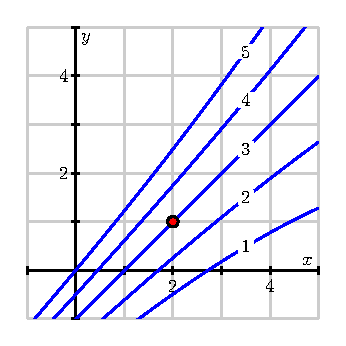
\includegraphics{figures/fig_10_3_activity_contour.eps}
      \end{center}
      \caption{Some contours of $f(x,y)$.}
      \label{F:10.5.contour}
    \end{figure}



  \ea

\end{activity} 

\begin{activitySolution}
\ba
\item According to the Chain Rule we have 
\begin{align*}
\frac{dz}{dt} &= \frac{\partial z}{\partial x} \frac{dx}{dt} + \frac{\partial z}{\partial y} \frac{dy}{dt} \\
	&= (2x+y^3)(-2\sin(t)) + (3xy^2)(2\cos(t)) \\
	&= -2(2\cos(t)+8\sin^3(t))\sin(t) + 48 \cos^2(t)\sin^2(t).
\end{align*}

\item 
	\begin{enumerate}[i.]
	\item We have
\begin{align*}
T_x(x,y) &= -2x \\
T_y(x,y) &= -8y,
\end{align*}
both measured in units of degrees Fahrenheit per foot. 
	\item In this situation we have $\frac{dx}{dt} = 2$ and $\frac{dy}{dt} = 0$. So 
\[\frac{dT}{dt} = -2x(2) -8y(0) = -4x.\]
Therefore, 
\[\frac{dT}{dt}\biggm|_{(2,0)} = -8 \frac{^{\circ}F}{\text{min}}.\]
	\item In this case we have 
\begin{align*}
\frac{dT}{dt} &= \frac{\partial T}{\partial x} \frac{dx}{dt} + \frac{\partial T}{\partial y} \frac{dy}{dt} \\	
	&= (-2x)(-6\sin(t)) - (8y)(3\cos(t)) \\
	&= 72\cos(t)\sin(t) - 72 \sin(t)\cos(t) \\
	&= 0.
\end{align*}
So
\[\frac{dT}{dt}\biggm|_{t=\pi/6} = 0 = \frac{dT}{dt}\biggm|_{t=\pi/4} =\frac{dT}{dt}\biggm|_{t=\pi/3}.\]
The fact that $\frac{dT}{dt} = 0$ means that $T$ is not changing, so on the path the ant is walking the temperature is constant. Note that 
\[T(6\cos(t), 3\sin(t)) = 100 - (36\cos^2(t) + 36\sin^2(t)) = 100-36 = 64,\]
so the ant is walking along a path of constant temperature $64^{\circ}F$. 
	\end{enumerate}
\item Since 
\[\frac{df}{dt}= \frac{\partial f}{\partial x} \frac{dx}{dt} + \frac{\partial f}{\partial y} \frac{dy}{dt},\]
we need to estimate $\frac{\partial f}{\partial x}$ and $\frac{\partial f}{\partial y}$ at $(2,1)$. Now
\begin{align*}
f_x(2,1) &\approx \frac{f(3,1) - f(1,1)}{2} \approx \frac{1.9-4.8}{2} = -1.45 \\
f_y(2,1) &\approx \frac{f(2,2) - f(2,0)}{2} \approx \frac{4.4-1.8}{2} = 1.3.
\end{align*}
The velocity vector at the point $(2,1)$ tells us $\frac{dx}{dt}$ and $\frac{dy}{dt}$ at the point $(2,1)$, so 
\[\frac{df}{dt}\biggm|_{(2,1)} \approx -1.45(-1) + 1.3(2) = 4.05.\]

\ea
\end{activitySolution}
\afterpa 